\documentclass{article}

\usepackage{amsmath}
\usepackage{graphicx}

\newcommand{\andSp}{\ \mathrm{and}\ }

\begin{document}
\title{APMA 4301: Problem Set 2}
\author{Brian Dawes}
\date{\today}
\maketitle
\section*{Problem 1}
\subsection*{a)}
Using the Taylor expansion, we can write:
\begin{equation}
u(x) = u(\bar x)+(x-\bar x)u'(\bar x)+\frac{(x-\bar x)^2}{2}u''(\bar x)+\frac{(x-\bar x)^3}{6}u^{(3)}(\bar x)
\end{equation}

Plugging in $x=0,h,2h$, we get:
\begin{eqnarray}
u_0 \approx u(\bar x)-\bar xu'(\bar x)+\frac{\bar x^2}{2}u''(\bar x)-\frac{\bar x^3}{6}u^{(3)}(\bar x) \\
u_1 \approx u(\bar x)+(h-\bar x)u'(\bar x)+\frac{(h-\bar x)^2}{2}u''(\bar x)+\frac{(h-\bar x)^3}{6}u^{(3)}(\bar x) \\
u_2 \approx u(\bar x)+(2h-\bar x)u'(\bar x)+\frac{(2h-\bar x)^2}{2}u''(\bar x)+\frac{(2h-\bar x)^3}{6}u^{(3)}(\bar x)
\end{eqnarray}
where $u_0=u(0)$, $u_1=u(h)$, and $u_2=u(2h)$.

Now we want to find stencil weights $s_0,s_1,s_2$ and $s_0',s_1',s_2'$ such that:
\begin{gather}
s_0u_0+s_1u_1+s_2u_2=u'(\bar x) \\
s_0'u_0+s_1'u_1+s_2'u_2=u''(\bar x)
\end{gather}

This can be represented in matrix form as:
\begin{equation}
\begin{bmatrix}
1 & 1 & 1 \\
-\bar x & h-\bar x & 2h-\bar x \\
\bar x^2/2 & (h-\bar x)^2/2 & (2h-\bar x)^2/2
\end{bmatrix}
\begin{bmatrix}
s_0 \\ s_1 \\ s_2
\end{bmatrix}
=
\begin{bmatrix}
0 \\ 1 \\ 0
\end{bmatrix}
\ \mathrm{or}\ 
\begin{bmatrix}
0 \\ 0 \\ 1
\end{bmatrix}
\end{equation}
which can be solved from the matrix:
\begin{equation}
\begin{bmatrix}
1 & 1 & 1 & 0 & 0\\
-\bar x & h-\bar x & 2h-\bar x & 1 & 0\\
\bar x^2/2 & (h-\bar x)^2/2 & (2h-\bar x)^2/2 & 0 & 1
\end{bmatrix}
\end{equation}

\subsubsection*{Case 1: $\bar x=0$}
Our matrix becomes:
\begin{align*}
\begin{bmatrix}
1 & 1 & 1 & 0 & 0\\
0 & h & 2h & 1 & 0\\
0 & h^2/2 & 2h^2 & 0 & 1
\end{bmatrix}
&\to
\begin{bmatrix}
1 & 1 & 1 & 0 & 0\\
0 & h & 2h & 1 & 0\\
0 & 0 & h^2 & -h/2 & 1
\end{bmatrix} \\
&\to s_2=-1/2h\andSp s_2'=1/h^2 \\
&\to s_1=2/h\andSp s_1'=-2/h^2 \\
&\to s_0=-3/2h\andSp s_0'=1/h^2
\end{align*}
\begin{equation}
\boxed{(s_0,s_1,s_2)=\frac{1}{2h}(-3,4,-1)\andSp(s_0',s_1',s_2')=\frac{1}{h^2}(1,-2,1)}
\end{equation}

\subsubsection*{Case 2: $\bar x=h/2$}
Our matrix becomes:
\begin{align*}
\begin{bmatrix}
1 & 1 & 1 & 0 & 0\\
-h/2 & h/2 & 3h/2 & 1 & 0\\
h^2/8 & h^2/8 & 9h^2/8 & 0 & 1
\end{bmatrix}
&\to\begin{bmatrix}
1 & 1 & 1 & 0 & 0\\
0 & h & 2h & 1 & 0\\
0 & 0 & h^2 & 0 & 1
\end{bmatrix} \\
&\to s_2=0\andSp s_2'=1/h^2 \\
&\to s_1=1/h\andSp s_1'=-2/h^2 \\
&\to s_0=-1/h\andSp s_0'=1/h^2
\end{align*}
\begin{equation}
\boxed{(s_0,s_1,s_2)=\frac{1}{h}(-1,1,0)\andSp(s_0',s_1',s_2')=\frac{1}{h^2}(1,-2,1)}
\end{equation}
\subsubsection*{Case 3: $\bar x=h$}
Our matrix becomes:
\begin{align*}
\begin{bmatrix}
1 & 1 & 1 & 0 & 0\\
-h & 0 & h & 1 & 0\\
h^2/2 & 0 & h^2/2 & 0 & 1
\end{bmatrix}
&\to
\begin{bmatrix}
1 & 1 & 1 & 0 & 0\\
-h & 0 & h & 1 & 0\\
0 & 0 & h^2 & h/2 & 1
\end{bmatrix} \\
&\to s_2=1/2h\andSp s_2'=1/h^2 \\
&\to s_0=-1/2h\andSp s_0'=1/h^2 \\
&\to s_1=0\andSp s_1'=-2/h^2
\end{align*}
\begin{equation}
\boxed{(s_0,s_1,s_2)=\frac{1}{2h}(-1,0,1)\andSp(s_0',s_1',s_2')=\frac{1}{h^2}(1,-2,1)}
\end{equation}

\subsection*{b)}
Since we already accounted for the first and second derivatives in the calculation of our stencil weights, our leading error can only come from the third derivative or higher terms in Eqns. 2, 3, and 4.

\subsubsection*{Case 1: $\bar x=0$}
For the first derivative, we get:
\begin{equation}
1/2h(0+2h^3/3-4h^3/3)u^{(3)}(0)=\boxed{-\frac{h^2}{3}u^{(3)}(0)}
\end{equation}
and for the second derivative, we get:
\begin{equation}
1/h^2(0-h^3/3+4h^3/3)u^{(3)}(0)=\boxed{hu^{(3)}(0)}
\end{equation}

\subsubsection*{Case 2: $\bar x=h/2$}
For the first derivative, we get:
\begin{equation}
1/h(h^3/48+h^3/48+0)u^{(3)}(h/2)=\boxed{-\frac{h^2}{24}u^{(3)}(h/2)}
\end{equation}
and for the second derivative, we get:
\begin{equation}
1/h^2(-h^3/48-h^3/24+9h^3/16)u^{(3)}(h/2)=\boxed{\frac{h}{2}u^{(3)}(h/2)}
\end{equation}

\subsubsection*{Case 3: $\bar x=h$}
For the first derivative, we get:
\begin{equation}
1/2h(h^3/6+0+h^3/6)u^{(3)}(h)=\boxed{\frac{h^2}{6}u^{(3)}(h)}
\end{equation}
and for the second derivative, we get:
\begin{equation}
1/h^2(h^3/6+0+h^3/6)u^{(3)}(h)=0
\end{equation}

Since the third derivative cancels out, we must look at the fourth derivative to find the leading error term. The fourth derivative error term is:
\begin{equation}
(h^4s0'/24+0+h^4s2'/24)u^{(4)}(h)=\boxed{\frac{h^2}{12}u^{(4)}(h)}
\end{equation}
\section*{Problem 2}
\subsection*{a)}
\subsubsection*{i.}
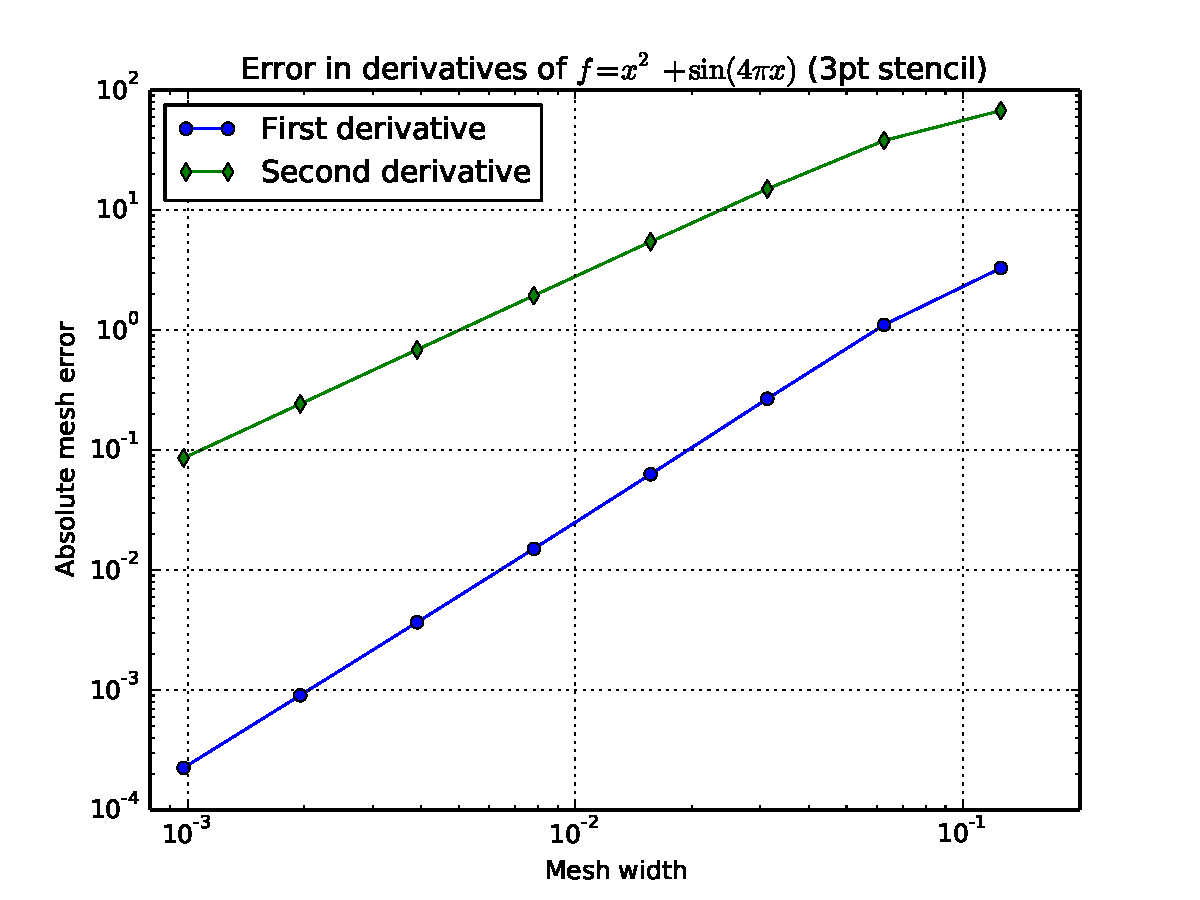
\includegraphics[width=\linewidth]{3PtStencilError.pdf}
\subsubsection*{ii.}
\subsubsection*{iii.}
\subsection*{b)}
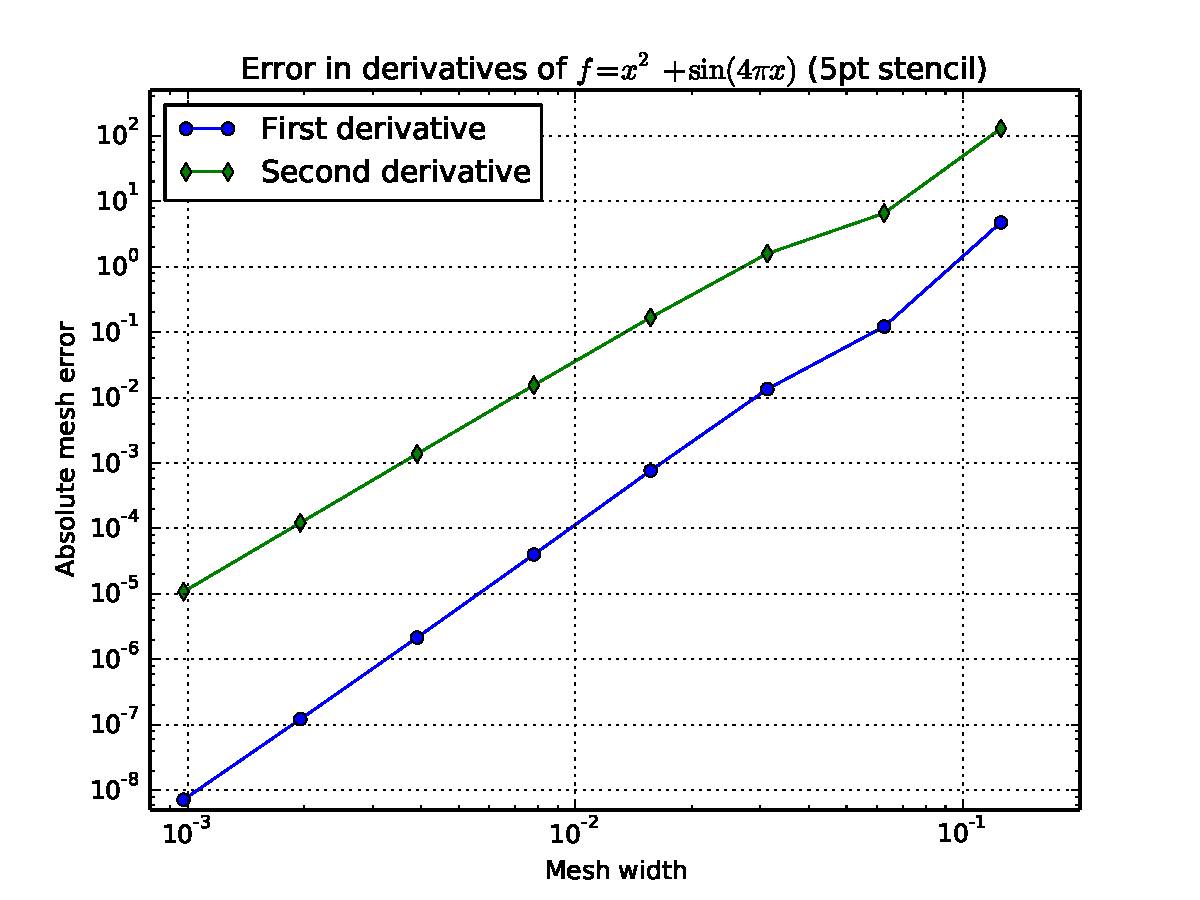
\includegraphics[width=\linewidth]{5PtStencilError.pdf}
\section*{Problem 3}
\subsection*{a)}
\subsection*{b)}
\subsection*{c)}
\end{document}